%% LyX 2.3.3 created this file.  For more info, see http://www.lyx.org/.
%% Do not edit unless you really know what you are doing.
\documentclass[twocolumn,english]{article}
\usepackage[T1]{fontenc}
\usepackage[latin9]{inputenc}
\usepackage{float}

\makeatletter
%%%%%%%%%%%%%%%%%%%%%%%%%%%%%% User specified LaTeX commands.
\usepackage{algorithm,algpseudocode}

\usepackage{tikz}
\usetikzlibrary{shapes, arrows}
\usetikzlibrary{er,positioning}
\usetikzlibrary{matrix}
\tikzset{
    events/.style={ellipse, draw, align=center},
}

\usepackage{pgfplots}

\makeatother

\usepackage{babel}
\usepackage[style=numeric]{biblatex}
\begin{document}
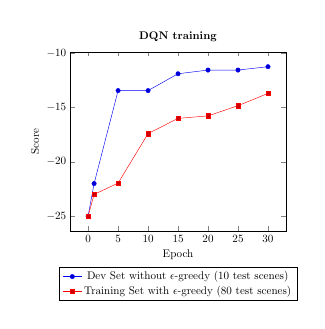
\begin{tikzpicture}[ scale=0.4]

	\begin{axis}[ xlabel=Epoch, ylabel=Score, title=\textbf{DQN training}, legend style={at={(0.5,-0.2)}, anchor=north}] 
		\addplot coordinates { (0, -25) (1, -22) (5, -13.44) (10, -13.44)  (15, -11.89) (20, -11.55) (25, -11.55) (30, -11.24)};
		\addplot coordinates { (0, -25) (1, -23) (5, -21.96) (10, -17.4)   (15, -16.0)  (20, -15.77) (25, -14.83) (30, -13.70) };

		\legend{Dev Set without $\epsilon$-greedy (10 test scenes), Training Set with $\epsilon$-greedy (80 test scenes)}
	\end{axis}
\end{tikzpicture}


\end{document}
